
% Chapter 3

\chapter{État de l'art} % 3rd chapter title

\label{Chapter3} % For referencing the chapter elsewhere, use \ref{Chapter3} 


%----------------------------------------------------------------------------------------

\section{Position du problème}
\label{sec:position}

Nous commençons par présenter une modélisation mathématique d'une plaque de glace (appelé floe) sur la mer. Six variables (locales) sont nécessaires pour décrire le floe occupant la région fermée de l'espace $\Omega$ (voir \cref{fig:floe}) :
\begin{itemize}
    \item Un ouvert connexe $\omega \in \Rdeux$ décrivant la section longitudinale du floe ;
    \item Deux fonctions $\hplus, \hmoins \in \mathcal{F}(\omega, \Run)$ décrivant l'épaisseur du floe, telle que $\forall x \in \omega, \hmoins(x) \leq \hplus(x)$ ;
    \item Le centre de masse du floe $G(w)$ ;
    \item Deux vecteurs $\eun$ et $\edeux$ formant une base sur $\omega$.
\end{itemize}

\begin{figure}[!h]
    \centering
    \begin{subfigure}[b]{0.45\textwidth}
        \centering
        % 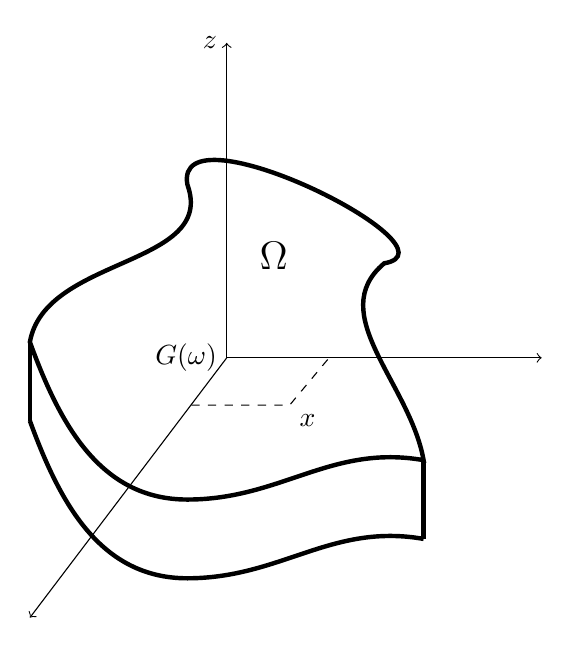
\begin{tikzpicture}
\node[coordinate] (v1) at (-3,3) {};
\node[coordinate] (v2) at (-5,1) {};
\node[coordinate] (v3) at (-3,-1) {};
\node[coordinate] (v4) at (0,-0.5) {};
\node[coordinate] (v5) at (-0.5,2) {};
%\draw  plot[smooth cycle, tension=.7] coordinates {(v5) (v1) (v2) (v3) (v4) (v5)};

\draw [ultra thick] (v1) to [out=290, in=80] (v2) to[out=290, in=180] (v3) to[out=0,in=170] (v4) to[out=100,in=220] (v5) to[out=10,in=100] (v1);

\node[coordinate] (v6) at (-5,0) {};
\node[coordinate] (v7) at (-3,-2) {};
\node[coordinate] (v8) at (0,-1.5) {};

\draw [ultra thick] (v2)--(v6); \draw [ultra thick] (v4)--(v8);
\draw [ultra thick]  (v6) to[out=290, in=180] (v7) to[out=0,in=170] (v8);

\node[coordinate] (v9) at (-2.5,0.8) {};
\node[coordinate] (v10) at (-5.0,-2.5) {};
\node[coordinate] (v11) at (1.5,0.8) {};
\node[coordinate] (v12) at (-2.5,4.8) {};

\draw [->] (v9)--(v10);
\draw [->] (v9)--(v11);
\draw [->] (v9)--(v12);


\node[left] (v9) at (-2.5,0.8) {$G(\omega)$};
\node[left] (v12) at (-2.5,4.8) {$z$};
\node[above left] (v13) at (-1.6,1.8) {\Large $\Omega$};

\node[coordinate] (v14) at (-1.2,0.8) {};
\node[coordinate] (v15) at (-1.7,0.2) {};
\node[coordinate] (v16) at (-2.95,0.2) {};
\draw[dashed] (v16)--(v15)--(v14);

\node[below right] (v15) at (-1.7,0.2) {$x$};

\end{tikzpicture}
        \includegraphics[width=.8\textwidth]{FloeVue1.tikz} 
        \caption{Vue d'un floe}
        \label{fig:floe1}
    \end{subfigure}
    % \hfill
    \begin{subfigure}[b]{0.45\textwidth}
        \centering
        % \usetikzlibrary{patterns}

\begin{tikzpicture}

\node[coordinate] (v0) at (0,0) {};
\node[coordinate] (v1) at (-5,0) {};
\node[coordinate] (v2) at (5,0) {};
\node[coordinate] (v3) at (0,-5) {};
\node[coordinate] (v4) at (0,5) {};

\draw [->] (v1)--(v2);
\draw [->] (v3)--(v4);

\node (v5) at (-4,2.5) {};
\node (v6) at (-1.5,3.5) {};
\node (v7) at (1,3.5) {};
\node (v8) at (3,2.5) {};
\node (v9) at (4,2.5) {};
\node (v10) at (-3.5,-2.5) {};
\node (v11) at (-2,-3.5) {};
\node (v12) at (-0.5,-3) {};
\node (v13) at (0.5,-3) {};
\node (v14) at (2,-3.5) {};
\node (v15) at (4.5,-3.5) {};

\draw[ultra thick]  plot[smooth, tension=.7] coordinates {(v5) (v6) (v7) (v8) (v9)};
\draw[ultra thick]  plot[smooth, tension=.7] coordinates {(v10) (v11) (v12) (v13) (v14) (v15)};

\draw [white, pattern=north east lines, xshift=0.5cm,yshift=4.5cm] plot coordinates {(v5) (v6) (v7) (v8) (v9) (v15) (v14) (v13) (v12) (v11) (v10) (v5)};

\node [above right] at (0,3.5) {\Large \bfseries $h_{+}(x)$};
\node [below right] at (0,-3.5) {\Large \bfseries $h_{-}(x)$};
\node [right] at (5,0) {\Large \bfseries $x$};
\node [left] at (0,5) {\Large \bfseries $z$};

\end{tikzpicture} 
        \includegraphics[width=.8\textwidth]{FloeVue2.tikz} 
        % \includegraphics[width=2cm]{Figures/FloeVue2.tex}
        \caption{Coupe transversale}
        \label{fig:floe2}
    \end{subfigure}
       \caption{Illustration de la géométrie d'un floe de glace $\Omega$.}
       \label{fig:floe}
\end{figure}

\noindent On confond le floe au volume qu'il occupe dans l'espace $\Omega$ :
\[
    \Omega = \{(x,z) \,|\, x \in \omega \in \Rdeux, \, z \in \,]\hmoins(x), \hplus(x)[ \, \} \,.
\] 
Les fonctions $\hmoins$ et $\hplus$ permettent de définir trois quantités (voir \cref{fig:h}) :
\begin{itemize}
    \item L'épaisseur moyenne du floe : $\bar{h} =  \sup_{x\in\omega}{\hplus(x)} - \inf_{x\in\omega}{\hmoins(x)}$ ;
    \item La plus forte épaisseur : $\bar{h}^* = \sup_{x\in\omega}{ \vert \hplus(x) - \hmoins(x) \vert}$ ;
    \item La plus faible épaisseur : $\underline{h}^* = \inf_{x\in\omega}{ \vert \hplus(x) - \hmoins(x) \vert}$. 
\end{itemize}

\begin{figure}[!h]
    \centering
    % \begin{tikzpicture}
	\begin{pgfonlayer}{nodelayer}
		\node [style=none] (0) at (0, 0) {};
		\node [style=none] (1) at (0, 5) {};
		\node [style=none] (2) at (0, -5) {};
		\node [style=none] (3) at (10, 0) {};
		\node [style=none] (4) at (-10, 0) {};
		\node [style=none] (5) at (-9.25, 2.5) {};
		\node [style=none] (6) at (-3.5, 1.5) {};
		\node [style=none] (7) at (3.25, 1.25) {};
		\node [style=none] (8) at (8.75, 4.75) {};
		\node [style=none] (9) at (-9, -6.75) {};
		\node [style=none] (10) at (-5, -4) {};
		\node [style=none] (11) at (2.5, -1.75) {};
		\node [style=none] (12) at (8.75, -1.25) {};
	\end{pgfonlayer}
	\begin{pgfonlayer}{edgelayer}
		\draw [->] (1.center) to (2.center);
		\draw [->] (4.center) to (3.center);
		\draw [bend right=15, looseness=0.75] (5.center) to (6.center);
		\draw [in=-165, out=0, looseness=1.25] (6.center) to (7.center);
		\draw [in=-135, out=15, looseness=1.25] (7.center) to (8.center);
		\draw [in=-165, out=45] (9.center) to (10.center);
		\draw [in=195, out=0, looseness=0.50] (10.center) to (11.center);
		\draw [in=180, out=15, looseness=0.75] (11.center) to (12.center);
	\end{pgfonlayer}
\end{tikzpicture}

    \includegraphics[width=.6\textwidth]{h.tikz}
    \caption{Différentes épaisseurs décrivant un floe de glace. Pour l'instant, afin d'obtenir un floe relativement plat (i.e $\bar{h}$ faible), $\hmoins$ sera pris identiquement nul, et $\hplus$ constant.}
    \label{fig:h}
\end{figure}

\noindent Les vecteurs $\eun$ et $\edeux$ sont liés à $\omega$, et pointent vers un point fixe du bord $\partial \omega$ du floe c-à-d :
\[
    \exists \sigma_i \in \partial \omega \, | \, e_i(\omega) = \frac{\sigma_i - G(\omega)}{\Vert \sigma_i - G(\omega) \Vert}, \text{ pour } i \in \{1,2\} \,,
\]
où $\Vert \cdot \Vert$ désigne la norme euclidienne de $\Rdeux$. Notons que $\sigma_1 \neq \sigma_2$, et $\eun \cdot \edeux = 0$ de façon à ce que la base orthonormée $(\eun, \edeux)$ soit directe.

Un floe $\Omega = (\omega, \eun, \edeux, G(\omega), \hmoins, \hplus)$ se déplace sur la mer\footnote{Pour l'instant, la mer est considérée comme un ouvert dans $\Rdeux$. Plus tard, nous prendrons en compte sont épaisseur lorsque nous la modéliserons par une sphère de $\Rtrois$.} $\mathcal{M} \in \Rdeux$. Au temps $t$ après une translation de vecteur $u(t)$ (et de matrice $\mathsf{T}_{u(t)}$), et une rotation de vecteur $\theta(t)$ (et de matrice $\bmat{R}_{\theta(t)}$), on obtient le floe $\Omega (t)$ défini par :
\[
    \Omega (t) = (\omega^\prime, \bvec e^1(\omega^\prime), \bvec e^2(\omega^\prime), G(\omega^\prime), \hmoins, \hplus) \,,
\]
avec
$$ 
\begin{cases}
    \omega^\prime = \bmat{T}_{u(t)} \bmat{R}_{\theta(t)} \omega \,, \\
    \bvec e_1(\omega^\prime) = \bmat{T}_{u(t)} \bmat{R}_{\theta(t)} \bvec e_1(\omega) \,, \\
    \bvec e_2(\omega^\prime) = \bmat{T}_{u(t)} \bmat{R}_{\theta(t)} \bvec e_2(\omega) \,, \\
    G(\omega^\prime) = \bmat{T}_{u(t)} \bmat{R}_{\theta(t)} G(\omega) \,.
\end{cases}
$$
C'est cette dernière notation mettant en exergue la dépendance avec le temps que nous utiliserons tout au long de ce rapport.

% \begin{figure}[!h]
%     \centering
%     % \begin{tikzpicture}
	\begin{pgfonlayer}{nodelayer}
		\node [style=none] (0) at (0, 0) {};
		\node [style=none] (1) at (0, 5) {};
		\node [style=none] (2) at (0, -5) {};
		\node [style=none] (3) at (10, 0) {};
		\node [style=none] (4) at (-10, 0) {};
		\node [style=none] (5) at (-9.25, 2.5) {};
		\node [style=none] (6) at (-3.5, 1.5) {};
		\node [style=none] (7) at (3.25, 1.25) {};
		\node [style=none] (8) at (8.75, 4.75) {};
		\node [style=none] (9) at (-9, -6.75) {};
		\node [style=none] (10) at (-5, -4) {};
		\node [style=none] (11) at (2.5, -1.75) {};
		\node [style=none] (12) at (8.75, -1.25) {};
	\end{pgfonlayer}
	\begin{pgfonlayer}{edgelayer}
		\draw [->] (1.center) to (2.center);
		\draw [->] (4.center) to (3.center);
		\draw [bend right=15, looseness=0.75] (5.center) to (6.center);
		\draw [in=-165, out=0, looseness=1.25] (6.center) to (7.center);
		\draw [in=-135, out=15, looseness=1.25] (7.center) to (8.center);
		\draw [in=-165, out=45] (9.center) to (10.center);
		\draw [in=195, out=0, looseness=0.50] (10.center) to (11.center);
		\draw [in=180, out=15, looseness=0.75] (11.center) to (12.center);
	\end{pgfonlayer}
\end{tikzpicture}

%     \includegraphics[width=.4\textwidth]{FloeMer.tikz}
%     \caption{Illustration du mouvement d'un floe de glace $F$ dans la mer, après une translation de vecteur $u(t)$ et une rotation d'angle $\theta(t)$, pour obtenir le floe $F_t$. On observe la transformation des propriétés du floe, en partucilier les vecteurs $e_1(\omega)$ et $e_2(\omega)$ qui restent liés au floe.}
% \end{figure}


Lors de leur mouvements sur la surface de la mer, les floes se fracturent sous l'effet des vents et des courants océaniques, des phénomènes thermodynamiques, etc. Nous nous intéresserons donc au phénomène de percussion en vue de l'initialisation des fractures dans les floes de glace. Afin de décrire le mouvement des floes de glace sur la mer, nous devons nous munir d'un repère absolu, que nous notons $\mathcal{R}_{abs} = (O, \bvec i, \bvec j, \bvec k)$. Le repère associé au floe $\Omega_i$ sera noté $\mathcal{R}_{\Omega_i} = (O, \bm \eun, \bvec \edeux, \bvec k)$. Dans ce repère absolu, le floe possède 3 degrés de libertés : l'abscisse et l'ordonné de son centre de gravité $G_i(\omega)$, et son orientation donnée par l'angle $\theta_i (t)$ (voir \cref{fig:FloeRepere}). 

\begin{figure}[!h]
    \centering
    % \begin{tikzpicture}
	\begin{pgfonlayer}{nodelayer}
		\node [style=none] (0) at (0, 0) {};
		\node [style=none] (1) at (0, 5) {};
		\node [style=none] (2) at (0, -5) {};
		\node [style=none] (3) at (10, 0) {};
		\node [style=none] (4) at (-10, 0) {};
		\node [style=none] (5) at (-9.25, 2.5) {};
		\node [style=none] (6) at (-3.5, 1.5) {};
		\node [style=none] (7) at (3.25, 1.25) {};
		\node [style=none] (8) at (8.75, 4.75) {};
		\node [style=none] (9) at (-9, -6.75) {};
		\node [style=none] (10) at (-5, -4) {};
		\node [style=none] (11) at (2.5, -1.75) {};
		\node [style=none] (12) at (8.75, -1.25) {};
	\end{pgfonlayer}
	\begin{pgfonlayer}{edgelayer}
		\draw [->] (1.center) to (2.center);
		\draw [->] (4.center) to (3.center);
		\draw [bend right=15, looseness=0.75] (5.center) to (6.center);
		\draw [in=-165, out=0, looseness=1.25] (6.center) to (7.center);
		\draw [in=-135, out=15, looseness=1.25] (7.center) to (8.center);
		\draw [in=-165, out=45] (9.center) to (10.center);
		\draw [in=195, out=0, looseness=0.50] (10.center) to (11.center);
		\draw [in=180, out=15, looseness=0.75] (11.center) to (12.center);
	\end{pgfonlayer}
\end{tikzpicture}

    \includegraphics[width=.5\textwidth]{FloeRepere.tikz}
    \caption{Positionnement d'un floe de glace $\Omega_i$ dans le repère absolu $\mathcal{R}_{abs}$.}
    \label{fig:FloeRepere}
\end{figure}


%----------------------------------------------------------------------------------------

\section{Résumé de thèse de M. Rabatel}

Une fois le modèle défini, il nous faut établir les équations décrivant la dynamique du floe, et celle de son environnement. Les travaux de \citeauthor{rabatel2015thesis} (et plus tard ceux de \citeauthor{balasoiu2020thesis}) ont extensivement traité le problème de modélisation dynamique et de simulation d'un assemblage de floe de glace. Nous résumons ici les principales idées de son raisonnement, tout en présentant l'état de l'art dans ce domaine.

\subsection{Modélisation théorique de la dynamique des glaces de mer}

\subsubsection{La cinétique du floe}

L'approche discrète décrite dans \parencite{rabatel2015thesis} utilise les mêmes notations que celles présentées à la \cref{sec:position}. Les obstacles\footnote{Nous faisons allusion aux obstacles au déplacement des floes. Il peut s'agir des iles, des stations offshore, etc.} sont des floes aux mêmes propriétés que les floes de glace, à la seule différence qu'ils ont une masse (volumique) infinie. Dans \parencite{rabatel2015thesis}, l'auteur travaille dans un repère orthonormé direct $\mathcal{R}_{abs} = (O, \bvec i, \bvec j, \bvec k)$ ; cependant, vu que la mer est considérée plane, le mouvement du floe peut être décrit dans le plan $\mathcal{P} = (O, \bvec i, \bvec j)$. Ensuite, \citeauthor{rabatel2015thesis} désigne la vitesse angulaire du floe $\Omega_i$ par 
$$
\bvec{\uptheta}_i(t) = \theta_i(t)\bvec{k} = (0,0,\theta_i(t))^T \,.
$$
Soit $P$ (de coordonné $x$) un point quelconque de $\P \subset \Rdeux$. Sa vitesse dans le repère $\R_{abs}$ est donnée est donnée par la formule de Varignon :
$$
\dot{P}(t) = \dot{G}_i(t) + \bm{\uptheta}_i(t) \wedge \bvec{G_iP} \,,
$$
où le symbole $\wedge$ représente le produit vectoriel dans $\Rtrois$. La masse (constante) du floe rigide indéformable est donnée par 
$$
M_i = \rho_i \int_{\Omega_i(t)} h_{i, +} (x) \diff x \,.
$$
Ensuite, l'auteur défini :
\begin{itemize}
    \item la somme des forces par unité de volume qui s'applique au centre de masse du floe $\Omega_i$ : $$\bvec{F}_i = \rho_i \int_{\Omega_i(t)} \bvec{F}(x) \diff x \,,$$
    \item le moment cinétique\footnote{Il s'agit d'un moment dû à l'accélération du floe ; alors que le moment dynamique est dû aux forces extérieures. Notons que ces deux vecteurs sont portés par $\bvec{k}$, et peuvent donc être remplacé par des scalaires correspondants.} en $G$ : $$L_i = \rho_i \intO{i} \bvec{GP} \wedge \dot{\bvec{P}}(t) \diff x \,,$$
    \item le moment dynamique en $G$ : $$\mathfrak{M}_i = \intO{i} \bvec{GP} \wedge \bvec{F}(x) \diff x \,.$$
\end{itemize}
Sous le formalisme de Newton-Euler, \citeauthor{rabatel2015thesis} montre que chaque floe $\Omega_i$ vérifie :
$$
% \begin{align}
    \begin{cases}
        M_i \frac{\diff \dot{\bvec{G}}_i(t)}{\diff t} &= \bvec{F}_i \\
        \mathcal{I}_i \frac{\diff \dot{\theta}_i(t)}{\diff t} &= \mathfrak{M}_i
    \end{cases} \,,
% \end{align}
$$
où $\mathcal{I}_i$ représente le moment d'inertie du floe $i$. Ce système se réécrit facilement sous la forme 
\begin{align}    
    \mathcal{M}_i \frac{\diff W_i(t)}{\diff t} = \mathcal{H}_i(t) \,,
\end{align}
avec 
$$
\mathcal{M}_i = 
\begin{pmatrix}
    M_i & 0 & 0 \\ 0 & M_i & 0 \\ 0 & 0 & \mathcal{I}_i
\end{pmatrix} \,, \quad
W_i(t) = 
\begin{pmatrix}
    \dot{\bvec{G}}(t) \\ \dot{\theta}_i(t)
\end{pmatrix} \,,
\text{ et } \quad \mathcal{H}_i(t) = 
\begin{pmatrix}
    \bvec{F}_i(t) \\ \mathfrak{M}_i(t)
\end{pmatrix} \,.
$$
Pour un système $S$ composé de $n$ floes, le problème précédent doit être satisfait pour tous les floes. \parencite[p.18]{rabatel2015thesis} montre que cela revient à résoudre l'équation
\begin{align} \label{eq:bilan1}
    \mathcal{M} \frac{\diff W(t)}{\diff t} = \mathcal{H}(t) \,,
\end{align}
avec 
$$
\mathcal{M} = (\mathcal{M}_i)_{1\leq i \leq n } \,, \quad
\mathcal{W}(t) = (\mathcal{W}_i(t))_{1\leq i \leq n } \,, \text{ et } \quad
\mathcal{M}(t) = (\mathcal{M}_i(t))_{1\leq i \leq n }  \,.
$$
L'énergie cinétique du floe $\Omega_i$ quant à elle sera donné par :
$$
E_i(t) = \frac{1}{2}M_i \dot{G}_i(t)^2 + \frac{1}{2}\mathfrak{I}_i \dot{\theta}_i(t)^2 \,. 
$$ 


\subsubsection{L'interaction entre les floes}


Le domaine de la mécanique du contact s'est grandement développé ces derniers siècles, avec plusieurs scientifiques qui ont tenté de décrire le phénomène de contact entre des corps rigides. Notons que le problème d'interaction entre les floes est un problème de \textbf{dynamique non-régulière} (contrairement au problème de déplacement des floes entre deux collisions qui lui, est un problème de \textbf{dynamique régulière}). Dans \parencite{rabatel2015thesis}, l'auteur considère deux lois de contact afin de décrire les phénomènes qui se produisent de façon précise :
\begin{itemize}
    \item Une \textbf{condition unilatérale de Signorini} : afin de décrire la condition de non-interpénétration ; cette condition est portée par la composante normale\footnote{La composante normale permet aussi d'assurer la dissipation de l'énergie à travers \textbf{la loi de Poisson}.} de la force de contact\footnote{La force de contact est la somme d'une friction tangentielle, et d'une réaction normale.} lors de la collision.
    \item Une \textbf{loi de friction de Coulomb} : afin de modéliser le comportement de friction pendant une collision. Cette condition est portée par la composante tangentielle de la force de contact.
\end{itemize}

\noindent Afin de traiter ces problèmes de contact, deux approches principales ont été d'enveloppées par les scientifiques : l'approche non-régulière et l'approche de régularisation des lois de contact. 

Parmi les pionniers dans l'\textbf{approche de régularisation} pour la résolution de la condition unilatérale de Signorini, nous pouvons citer Hertz ; Nevins et Whitney \parencite{nevins1972force,whitney1977force}, Moore \parencite{moore1988collision} ; Ces méthodes se sont largement répandues dans les études liées à la robotique, à la réalité virtuelle ou encore dans les opérations assistées par ordinateur, pour simuler un grand nombre d’objets en contact en petites ou grandes déformations, comme des habits, des cheveux ou encore des organes (voir \parencite{witkin1990fast,volino1995versatile,baraffandrew,raghupathi2004intestinal}). Concernant la seconde, la loi de friction de Coulomb, la discontinuité entre les phases de glissement et non-glissement a été traitée de différentes façons ; en utilisant la notion de coefficient de restitution, ou des modèles masse-ressorts. 
 
L'\textbf{approche non-régulière} a été développée en utilisant les concepts d'inclusion différentielles ; ceci afin de traiter la condition de Signorini. Moreau \parencite{moreau1985standard}, Aubin \parencite{aubin2012differential} et Monteiro Marques \parencite{monteiro1985chocs}, ont montré des résultats d’existence et d’unicité de solutions du problème sans friction. Puis, des résultats similaires ont été établis pour le contact unique avec friction (voir \parencite{moreau1986dynamique,monteiro1988inclusoes,panagiotopoulos2012inequality,jean1985system,monteiro1994existence}). Cependant, cette notion d'inclusion différentielle est difficile à manipuler ; c'est, d'après \citeauthor{rabatel2015thesis} la raison pour laquelle le problème du contact multiple avec friction reste encore très peu traité. Il a donc fallu attendre les années 80 avec l'essor des méthodes LCP pour donner un nouveau souffle à l'approche non régulière. Nous pouvons citer ici les travaux de Lötstedt qui fournit des preuves d’existence et d’unicité pour le contact avec la friction de Coulomb (voir \parencite{lotstedt1981coulomb,lotstedt1982mechanical,lotstedt1982time}). On cite aussi Klarbring et Pang, pour leur apport sur le plan des méthodes de programmations. \parencite{rabatel2015thesis} a opté pour cette approche car elle facilite la construction des solutions à partir d’algorithmes tels que ceux de Lemke (voir \parencite{lemke1978some}). \citeauthor{rabatel2015thesis} s'inspire aussi des travaux de Baraff \parencite{baraff1993issues}, qui écrit les forces de contact dans les repères locaux aux points de contact. Ces repères sont définis par la normale et la tangente aux points de contact. La condition de complémentarité se résume comme ceci : "\textit{S’il y a contact alors la réaction est strictement positive et l’accélération relative nulle, et s’il n’y a pas contact l’accélération relative est strictement positive et la réaction nulle.}". Cependant, les travaux de Baraff sur l'existence de solutions sont limités par l'approche accélération-force, et le coefficient de friction qui sont utilisés. En utilisant des formulations en vitesse et impulsion, les chercheurs ont réussi à démontrer l’existence de solutions pour toute configuration à contacts multiples avec n’importe quel coefficient de friction.


Pour traiter le problème de collision entre les floes, les glaciologues retiennent une multitude de modèles principalement intégrés aux milieux continus. Par exemple, dans les articles de Solomon \parencite{solomon1970study}, ceux de Hibler \parencite{hibler1979dynamic} et ceux de Bratchie \parencite{bratchie1984rheology}, la force résultante des interactions est due à une contrainte interne. On note aussi les modèles basés sur théorie des flux de particules. Dans \parencite{shen1986applying,hopkins1985collisional} par exemple, les collisions ne sont pas détectées précisément et les paramètres décrivant la collision sont déterminés par une méthode de Monte Carlo. L'introduction de ces déformations dans les modèles discrets de la banquise a été initié dans les années 90 par Hopkins \parencite{hopkins1996mesoscale}, et récement par Herman et Wilchinsky \parencite{herman2011molecular,wilchinsky2010effect}. Cependant, elles sont basées sur la régularisation des lois de contact. Avant les travaux de \citeauthor{rabatel2015thesis}, il n'existait pas de modèle discret de banquise en utilisant une dynamique du contact non régulière.


Le modèle décrit par \parencite[p.5892]{rabatel2015dynamics} utilise deux conditions de complémentarité pour déterminer les vitesses des floes après le contact. La première est une condition de Signorini \parencite{signorini1933sopra} pour s'assurer de la non-interpénétration\footnote{Deux floes s'interpénètre si la "distance" entre ces deux floes est négative.} des floes. Pour décrire ces conditions, il faut au préalable écrire le problème de contact entre floes comme un problème implicite, où les inconnus sont les impulsions après le choc\footnote{Contrairement aux lois de contacts explicites (Hertz, Hooke, Coulomb), les lois implicites ne nécessitent pas la connaissance de la nature du contact entre les floes (glissement ou accroche).}. Pour cette deuxième condition de complémentarité, \citeauthor{rabatel2015thesis} se base sur les travaux de Stewart et Trinkle \parencite{stewart1996implicit} afin d'en extraire une condition qui vérifie la loi de friction de Coulomb. Le problème résultant a ensuite été résolu en utilisant des algorithmes de Lemke. 

\begin{figure}[!h]
    \centering
    % \begin{tikzpicture}
	\begin{pgfonlayer}{nodelayer}
		\node [style=none] (0) at (0, 0) {};
		\node [style=none] (1) at (0, 5) {};
		\node [style=none] (2) at (0, -5) {};
		\node [style=none] (3) at (10, 0) {};
		\node [style=none] (4) at (-10, 0) {};
		\node [style=none] (5) at (-9.25, 2.5) {};
		\node [style=none] (6) at (-3.5, 1.5) {};
		\node [style=none] (7) at (3.25, 1.25) {};
		\node [style=none] (8) at (8.75, 4.75) {};
		\node [style=none] (9) at (-9, -6.75) {};
		\node [style=none] (10) at (-5, -4) {};
		\node [style=none] (11) at (2.5, -1.75) {};
		\node [style=none] (12) at (8.75, -1.25) {};
	\end{pgfonlayer}
	\begin{pgfonlayer}{edgelayer}
		\draw [->] (1.center) to (2.center);
		\draw [->] (4.center) to (3.center);
		\draw [bend right=15, looseness=0.75] (5.center) to (6.center);
		\draw [in=-165, out=0, looseness=1.25] (6.center) to (7.center);
		\draw [in=-135, out=15, looseness=1.25] (7.center) to (8.center);
		\draw [in=-165, out=45] (9.center) to (10.center);
		\draw [in=195, out=0, looseness=0.50] (10.center) to (11.center);
		\draw [in=180, out=15, looseness=0.75] (11.center) to (12.center);
	\end{pgfonlayer}
\end{tikzpicture}

    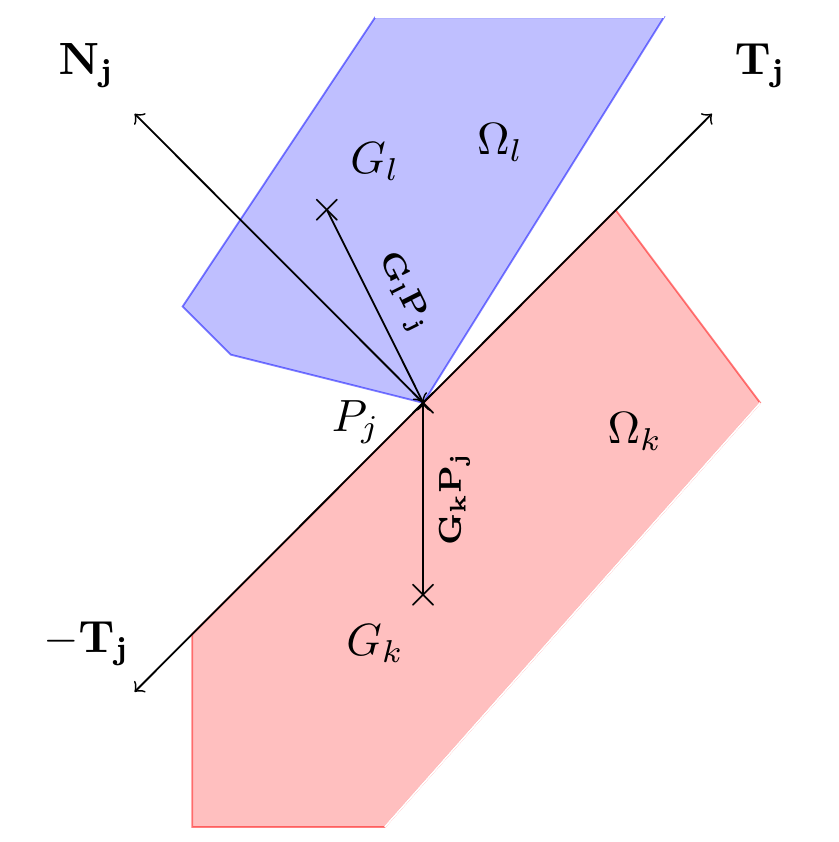
\includegraphics[width=.28\textwidth]{Collision1.png}
    \caption{Interaction entre deux floes $\Omega_k$ et $\Omega_l$ au point $P_j$ \parencite[p.26]{rabatel2015thesis}.}
    \label{fig:Collision1}
\end{figure}

Soit $P_j$, ($j \in \{1,\ldots,n\}$) un point de contact entre les floes $\Omega_k$ et $\Omega_l$ (voir \cref{fig:Collision1}). Nous notons $\bvec{F}_{kj}(t)$ la force de contact du floe $\Omega_k$ au floe $\Omega_l$ appliquée en $P_j$. Par convention, une matrice de contact $\bmat{M_c}$ est définie telle que son coefficient $c_kj$ vaut :
\begin{itemize}
    \item $0\,\,\,\,\,\, $ si le point de contact $P_j$ n’est pas un point de contact du floe $\Omega_k$ ;
    \item $-1$ si le point de contact $P_j$ est un point de contact entre les floes $\Omega_k$ et $\Omega_l$ avec $k < l$ ;
    \item $1\,\,\,\,\,\, $ si le point de contact $P_j$ est un point de contact entre les floes $\Omega_k$ et $\Omega_l$ avec $k > l$.
\end{itemize}
En notant $E_k$ l’ensemble des points de contact du floe $\Omega_k$ au temps $t$, \parencite[p.26]{rabatel2015thesis} définit la résultante des forces de contact $\bvec{F}^c_k(t)$, au floe $\Omega_k$ comme :
$$
\bvec{F}^c_k(t) = \sum_{j \in E_k} c_{jk} \bvec{F}_{kj}(t) \,.
$$
En rajoutent ces forces aux forces extérieures lors du bilan des forces à l'\cref{eq:bilan1}, pour un floe $\Omega_k(t)$, on obtient :
\begin{align} \label{eq:bilan1}
    \mathcal{M} \frac{\diff W(t)}{\diff t} = \mathcal{H}(t) + \sum_{j \in E_k} \begin{pmatrix}
        \bvec{F}_{kj}(t) \\ \bvec{G^kP_j} \wedge \bvec{F}_{kj}(t) 
    \end{pmatrix} \,.
\end{align}


\subsubsection{Formulation en problème linéaire de complémentarité}


Il existe deux principales manières de formuler le problème du contact entre deux solides rigides. L'auteur de \parencite{rabatel2015thesis} opte pour le formalisme vitesse-impulsion, au détriment du formalisme accélération-force. En effet, l’approche en \textbf{vitesse-impulsion} apporte l’avantage de pouvoir exprimer la force de friction de Coulomb directement par rapport à la vitesse. Il n’est pas nécessaire de connaître la nature du contact. Il nous faut donc définir les notions d'impulsion. Sur un intervalle de temps $\delta t^*$, s’il y a un contact entre les floes $\Omega_k$ et $\Omega_l$ au point $P_j$, nous dirons que le floe $\Omega_k$ a subi un choc provenant du floe $\Omega_l$ au point de contact $P_j$ caractérisé par l’impulsion :
$$
\bvec{\mathcal{I}}_{kj} = \int_{\delta t^*} c_{kj} \bvec{F}_{kj}(t) \diff t \,.
$$ 
\citeauthor{rabatel2015thesis} fait donc apparaître les impulsions dans les équations des moments \cref{eq:bilan1} pour le floe $\Omega_k$ sur l’intervalle temporel $\delta t^*$ :
$$
\mathcal{M}_k \int_{\dtstar} \dot{W}_k(t) \diff t = \int_{\dtstar} \mathcal{H}(t) \diff t + \sum_{j \in E_k} \begin{pmatrix}
    \bvec{\mathcal{I}}_{kj} \\ \bvec{G_kP_j} \wedge \bvec{\mathcal{I}}_{kj} 
\end{pmatrix} \,.
$$
En écrivant $\dtstar = [t^{-}, t^{+}]$, on peut donc introduire les inconnues $\beta$, $\lambda \in (\Rdeux)^m$ pour le problème de contact  
\begin{align}
    \mathcal{M} \left( W(t^{+}) - W(t^{-}) \right) = \int_{\dtstar} \mathcal{H}(t) \diff t + \bmat{B}\beta + \bmat{J}\lambda \,,
\end{align}
où $\bmat{B}$ et $\bmat{J}$ sont deux matrices de $(\Rtrois)^{n \times m}$telle que
\begin{align*}
    \bmat{B} = (d_{kj})_{\substack{1 \leq k \leq n \\ 1 \leq j \leq m}} \,, \quad d_{kj} = \,
    \begin{cases}
        0 \in \Rtrois &\text{ si } P_j \text{ n'est pas un point de contact de } \Omega_k \\
        \begin{pmatrix}
            c_{kj} \bvec{T}_{j} \\ c_{kj} \bvec{P}_j\bvec{G}_k \wedge \bvec{T}_j 
        \end{pmatrix} &\text{ si } P_j \text{ est un point de contact de } \Omega_k
    \end{cases} \,, \\
    \bmat{J} = (s_{kj})_{\substack{1 \leq k \leq n \\ 1 \leq j \leq m}} \,, \quad s_{kj} = \,
    \begin{cases}
        0 \in \Rtrois &\text{ si } P_j \text{ n'est pas un point de contact de } \Omega_k \\
        \begin{pmatrix}
            c_{kj} \bvec{N}_{j} \\ c_{kj} \bvec{P}_j\bvec{G}_k \wedge \bvec{N}_j 
        \end{pmatrix} &\text{ si } P_j \text{ est un point de contact de } \Omega_k
    \end{cases} \,.
\end{align*}
Les matrices $\bmat{B}$ et $\bmat{J}$ sont obtenues par décomposition des forces de contact dans le repère de contact $\mathcal{R}_{\Omega_j} = (P_j, \bvec{T}_j, \bvec{N}_j)$ (voir \cref{fig:Collision1}).

Comme précédemment mentionné, afin de modéliser la friction dans une collision qui respecte la loi de Coulomb, \parencite{rabatel2015thesis} se base sur les travaux de Stewart et Trinkle \parencite{stewart1996implicit} qui définissent une condition de complémentarité reliant la composante tangentielle $\beta_j$ de l'impulsion appliquée au point $P_j$, la composante normale $\lambda_j$, la vitesse relative tangentielle du point $P_j$ et le coefficient de friction $\mu$. On introduit le vecteur $\tilde{\beta}$ contenant les composantes de l'impulsion tangentielle dans chacune des directions possible de glissement $\bvec{T}_j$ et $-\bvec{T}_j$. Il devient alors possible de formuler le problème de contact (sur tout le système $S$) sans interpénétration par le problème linéaire de complémentarité :
\begin{align} \label{eq:bilan3}
\begin{cases} \,\,
    \begin{pmatrix}
        0 \\ \bvec{w} \\ \gamma \\ \sigma 
    \end{pmatrix} =  
    \begin{pmatrix}
        \mathcal{M} &  -\bmat{J} & -\bmat{D} & 0 \\
        \bmat{J}^T & 0 & 0 & 0 \\
        \bmat{D}^T & 0 & 0 & \bmat{H} \\
        0 & \mu & -\bmat{H}^T & 0
    \end{pmatrix} 
    \begin{pmatrix}
        W(t^+) \\ \lambda \\ \tilde{\beta} \\ \alpha
    \end{pmatrix} + 
    \begin{pmatrix}
        \int_{\delta t^*} \mathcal{H}(t) \diff t - \mathcal{M} W(t^{-}) \\ 0 \\ 0 \\ 0
    \end{pmatrix} \\ \quad
    \begin{pmatrix}
        \bvec{w} \\ \gamma \\ \sigma
    \end{pmatrix} \geq 0 \,, \quad
    \begin{pmatrix}
        \lambda \\ \tilde{\beta} \\ \alpha
    \end{pmatrix} \geq 0 \,, \quad
    \begin{pmatrix}
        \bvec{w} \\ \gamma \\ \sigma
    \end{pmatrix} \cdot
    \begin{pmatrix}
        \lambda \\ \tilde{\beta} \\ \alpha
    \end{pmatrix}  
     = 0 \,,
\end{cases}
\end{align}
avec
\begin{align*}
    &\bvec{w} = \bmat{J}^T W(t^+) \,, \quad
    \bmat{H}^T = (e_{ij})_{\substack{1 \leq i \leq m \\ 1 \leq j \leq 2m}} \,, \quad \tilde{\beta} = (\tilde{\beta}_j)_{1\leq j \leq m} \,, \quad \lambda = (\lambda_j)_{1 \leq j \leq m} \,, \\
    &\mu \text{ est la matrice diagonale de diagonale} (\mu_1,\dots, \mu_m) \,,\\
    &e_{ij} = \begin{cases}
        1 \text{   si } j = 2(i-1) + 1 \text{ ou } j=2(i-1) + 2 \\
        0 \text{   sinon} 
    \end{cases} \,,\\
    &D = (\bvec{B}_1 \vert - \bvec{B}_1 \vert \ldots \vert \bvec{B}_m \vert -\bvec{B}_m) \, \text{   avec } \bvec{B}_j \text{ la colonne } j \text{ de la matrice } \bmat{B} \,.
\end{align*}
Le problème consiste alors à trouver les vitesses après contact $W(t^{+})$, à l’aide des composantes inconnues tangentielle et normale des impulsions dans les repères de contact $(\tilde{\beta}\, \gamma)$, elles-mêmes inconnues du système.


\subsubsection{Consistance énergétique}


D'après l'auteur de \parencite[p.42]{rabatel2015thesis}, traiter le problème de contact à partir de lois non régulières ne permet pas d’obtenir des solutions satisfaisant à la fois la non-interpénétration, la friction de Coulomb et une consistance énergétique. En se focalisant sur la consistance énergétique, \citeauthor{rabatel2015thesis} a subdivisé le problème en deux : une phase de compression et une phase de décompression suivant la loi de Poisson. La \textbf{phase de compression} modélise la capacité maximale des floes à emmagasiner, par la déformation, une partie ou la totalité de l’énergie cinétique transmise lors du contact. L'impulsion normale $\lambda^c$ calculée durant cette phase (en résolvant le problème de complémentarité (\cref{eq:bilan3})) correspond a un coefficient de restitution $\varepsilon = 0$. Les impulsions obtenues durant cette phase correspondent à celles nécessaire pour éviter la non-interpénétration, et correspondent donc a une énergie cinétique maximale emmagasinée. La \textbf{phase de décompression} correspond à la restitution partielle ou complète de l’énergie cinétique emmagasinée par la déformation des floes. L’impulsion lors de cette phase, notée $\lambda^d$, est déterminée par $\lambda^d = \varepsilon \lambda^c$ (l’hypothèse de Poisson \parencite{glocker1995multiple}). Durant la phase de décompression, \citeauthor{rabatel2015thesis} a donc opté pour la consistance énergétique et la non-interpénétration avec la solution :
$$
W^N = (1 + \varepsilon)W^{c} - \varepsilon W(t^{-}) \,,
$$
où $W^c$ représente les vitesses des floes après la phase de compression, et $\varepsilon$ le coefficient de restitution pour les contacts considérés inélastiques.

% \subsubsection{Traitement des conditions aux bords}

\subsubsection{Le modèle de l'environnement}


L’environnement est l’ensemble des forces extérieures qui agissent sur les floes hormis les forces de contact qui sont décrites dans la partie précédente. Ces principales forces sont:
\begin{itemize}
    \item La force de Coriolis $\bvec{\mathfrak{F}}_c$ donnée pour un floe $\Omega_i(t)$ par:
    $$
    \bvec{\mathfrak{F}}_{c,i}(t) = -f\bvec{k} \wedge \dot{\bvec G}_i(t) \,,
    $$
    avec $f$ le paramètre de Coriolis et $\bvec{k}$ le vecteur dirigé vers le haut du repère absolu $\mathcal{R}_{abs}$.
    \item Les forces de trainée associées au vent $\bvec{\tau}_a(t)$ et celle associée à l'océan $\bvec{\tau}_w(t)$: 
    \begin{align*}
        \bvec{\tau}_a(t) &= \rho_a C_a \Vert \bvec{U}_a(t) \Vert \bvec{U}_a(t) \,, \\        
        \bvec{\tau}_w(t,P) &= \rho_w C_w \Vert \bvec{U}_w(t) - \dot{P}(t) \Vert \left(\bvec{U}_w(t) - \dot{P}(t) \right) \,,
    \end{align*}
    avec $\rho$ la masse volumique du fluide (l'indice $a$ pour l'air et $w$ pour l'eau) et $C$ un coefficient de traînée sans dimension (voir [HI86]) ; $\bvec{U}_a$, $\bvec{U}_w$, $\dot{P}(t)$ respectivement la vitesse du vent à l'interface glace/fluide, la vitesse du courant oceanique à l'interface glace/fluide, et la vitesse d'un point $P$ du floe. 
\end{itemize}

Le modèle de dynamique régulière définit en \cref{eq:bilan1} peut se voire expliciter:
\begin{align*}
    \begin{cases}
            M_i \frac{\diff \dot{\bvec{G}}_i(t)}{\diff{t}} &= M_i \mathfrak{F}_{c,i}(t) + \int_{\Omega_i(t)} \bvec{\tau}_a(t) + \bvec{\tau}_w(t,P) \diff s \,,\\
            \mathcal{I}_i \frac{\diff \dot{\theta}_i(t)}{\diff t} &= \int_{\Omega_i(t)} \bvec{G}_i\bvec{P} \wedge \left(\bvec{\tau}_a(t) + \bvec{\tau}_w(t,P)\right) \diff s \,.
    \end{cases}
\end{align*} 
L'algorithme décrivant en détail le processus de collision ainsi que la consistance énergétique se trouve à la page 43 du document \parencite{rabatel2015thesis}.


\subsection{Méthodes numériques et algorithmiques pour la résolution du problème}
 
\subsubsection{Discrétisation temporelle}

Pour simuler la dynamique des floes de glace soumis a des forces extérieures et possiblement des collisions, il faut intégrer la dynamique régulière (entre deux collisions), et la dynamique non régulière ; et il existe deux principales méthodes pour la discrétisation en temps dans de tels problèmes. La méthode \textit{\textbf{time-stepping}} (voir \parencite{acary2013projected} pour les schéma de Moreau \parencite{moreau1986dynamique,jean1999non}, et de Schatzman-Paoli \parencite{paoli2002numerical,paoli2002numerical2} par exemple, pour lesquels une convergence a pu être exhibée à partir de la convergence en graphe de Moreau \parencite{moreau1978approximation}) ; comparé aux autres méthodes, la méthode \textit{time-stepping} traite mieux les points d'accumulation \parencite[p.58]{rabatel2015thesis} ; et est plus performante sur des problèmes de multiples contacts. Cependant, \citeauthor{rabatel2015thesis} pour le schéma \textit{\textbf{event-driven}} pour sa précision dans la localisation des collisions et sa facilité de manipulation. En plus, elles permettent d’utiliser des schémas d’intégration existant d’ordre élevé pour des équations différentielles ordinaires. Le seuil de collision choisi est suffisamment grand pour éviter de traiter les collisions une par une. Le schéma utilisé pour intégrer l'équation \cref{eq:bilan1} est un schéma du type Euler explicite, pour sa facilité d’implémentation, sa facilité à prédire la localisation en espace et en temps des futures collisions et enfin, sa capacité à dépasser les problèmes de points d’accumulation. 

La simulation par la méthode \textit{event-driven} demande la définition d'un pas de temps maximal pour lequel le schéma reste stable. Le pas de temps $\Delta t_max$ sera utilisé si aucune collision n'est détectée entre les instants $t$ et l'instant $t + \Delta t_max$. En se référant au un modèle idéalisé 1D (voir \parencite[p.49]{rabatel2015thesis}), \citeauthor{rabatel2015thesis} distingue deux critères pour la stabilité du schéma numérique au temps $t$ :
\begin{itemize}
    \item lorsque la vitesse caractéristique des floes $V_c(t) = N_a \bvec{U}_a(t) + \bvec{U}_w(t)$ est constante sur l'intervalle de simulation $I$, alors pour :  
    \begin{align} \label{eq:dtmax1}
        \Delta t \leq \Delta t_{max} = \min{ \left(\frac{\rho}{2 \vert \bvec{U}_a(t) \vert \sqrt{\rho_a C_a \rho_w C_w}} \,, \,\frac{2K_t}{L_t} \right)}
    \end{align}
    avec 
    $$
    \text{avec } L_t = \rho^{-1} \rho_w C_w \left( N_a^2 \bvec{U}_a^2 + (N_a\bvec{U}_a + 2 \bvec{U}_w)^2 \right) \,, \text{et } K_t = \vert V_c(t) \vert \text{ constant, }
    $$
    le schéma est stable c-à-d. $\dot{\bvec{G}} (t + \Delta t) \in [-K_t, K_t] = [-K_{t + \Delta t}, K_{t + \Delta t}]$ ;
    \item lorsque les variations de $V_c(t)$ entraînent une augmentation de $K_t$ au cours du temps. La propriété de stabilité reste vérifiée car $$\dot{\bvec{G}} (t + \Delta t) \in [-K_t, K_t] \in [-K_{t + \Delta t}, K_{t + \Delta t}] \,;$$
    \item lorsque les variations de $V_c(t)$ entraînent une diminution stricte de $K_t$ au cours du temps, alors la condition de stabilité dans les deux cas précédents ne peut être vérifiée. \citeauthor{rabatel2015thesis} introduit donc une seconde définition de la stabilité pour traiter ce cas. Il remarque que pour 
    \begin{align} \label{eq:dtmax2}
    \Delta t_{max} \leq \begin{cases}
        \frac{-2x}{\tilde{L}_t^{-}} \text{  si  } x \in  ]-\infty, K_{t+\Delta t}] \\
        \frac{-2x}{-\tilde{L}_t^{+}} \text{  si  } x \in  ]K_{t+\Delta t}, +\infty]
    \end{cases}\end{align}
    avec \begin{align*} \tilde{L}_t^{-} =  \rho^{-1} \rho_w C_w \left[ N_a^2 \bvec{U}_a(t+\Delta t)^2 - (\bvec{U}_w(t + \Delta t) - x)^2 \right] \\ \tilde{L}_t^{+} =  \rho^{-1} \rho_w C_w \left[ N_a^2 \bvec{U}_a(t+\Delta t)^2 + (\bvec{U}_w(t + \Delta t) - x)^2 \right] \,,
     \end{align*}
    on a la diminution de la vitesse des floes.
\end{itemize} 
En conclusion, pour une vitesse infinitésimale initiale $\dot{G}(0) \in [-K_0, K_0]$, pour tout $t \in I$, et pour tout $\Delta t_{max}$ vérifiant les \cref{eq:dtmax1,eq:dtmax2}, nous avons les vitesses des floes majorées par :
$$
\max_{t \in I}{K_t}
$$
\citeauthor{rabatel2015thesis} choisi donc de prendre 
$$
\Delta t_{max} = \min{ \left( \frac{3}{4} \frac{ -2 \left( \max_{t \in I}{K_t} \right)}{ \max_{t \in I}{\tilde{L}_t^{-}}}, \frac{3}{4} \frac{2 \left( \max_{t \in I}{K_t} \right) }{ \max_{t \in I}{-\tilde{L}_t^{+}}}, \frac{\rho}{2 \left(  \max_{t \in I}{  \vert \bvec{U}_a(t) \vert } \right)  \sqrt{\rho_a C_a \rho_w C_w}} \right)}
$$
pour s'assurer que le modèle idéalisé vérifie les critères de stabilité définis. 
Notons que le procédé global d’intégration de la dynamique pour le modèle se situe à la figure 2.2 du document \parencite[p.60]{rabatel2015thesis}, le schéma est repris à la \cref{fig:Algo1}.

\begin{figure}[!h]
    \centering
    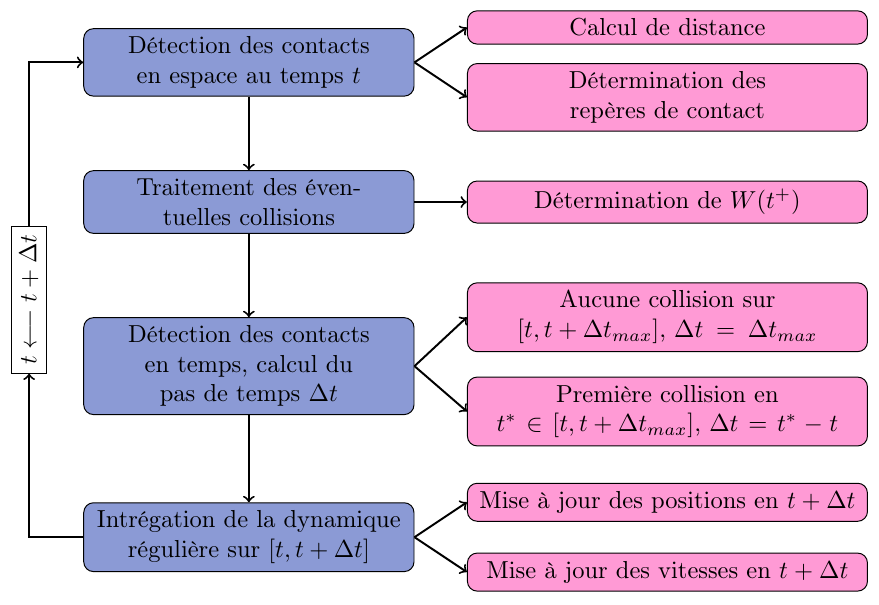
\includegraphics[width=.62\textwidth]{Algo1.png}
    \caption{Procédé global d’intégration de la dynamique pour notre modèle \parencite[p.60]{rabatel2015thesis}.}
    \label{fig:Algo1}
\end{figure}


\subsubsection{Détection des collisions en espace}

Des deux méthodes principales utilisées dans la littérature pour la détection des voisins, \citeauthor{rabatel2015thesis} a choisi la méthode de \textbf{hiérarchie de volumes englobants} pour sa facilité de mise en place et pour son efficacité même avec de grands ratios de tailles. L'alternative était la méthode de \textbf{partitionnement de l'espace} qui elle, souffre de plusieurs défauts non surmontables pour le modèle développé. Les méthodes de volumes englobants consistent à englober le contour de l’objet par des volumes à des échelles de plus en plus fines pour améliorer la détection.

\subsubsection{Détection des contacts en temps}

Il s'agit ici de trouver le pas de temps optimal c’est-à-dire un pas de temps $\Delta t$ pour lequel la configuration des floes ne contenant pas d’interpénétrations sur l’intervalle de temps $[t, t + \Delta t]$ et, pour tout $\varepsilon > 0$, contient au moins une interpénétration sur l’intervalle de temps $[t + \Delta t, t + \Delta t + \varepsilon]$ \parencite[p.87]{rabatel2015thesis}.
Lorsque le critère de collision n’est pas vérifié, \citeauthor{rabatel2015thesis} montre qu'il suffit de prendre 
$$
\Delta t_{i,j} = -\frac{-\delta_{i,j(t)} - tol_3}{\bvec{A}_{ij}(t) \cdot \left( \dot{G}_i(t) - \dot{G}_j(t) \right)} \,,
$$
avec 
$$
\bvec{A}_{i,j}(t) = \frac{C_{0,i}(t) - C_{0,i}(t)}{d\left(C_{0,i}(t), C_{0,i}(t) \right)} \,, \text{ et  } \quad tol_3 = \frac{\xi}{20} \,.
$$
Lorsque le critère de collision est vérifié, il faut plutôt prendre 
$$
\Delta t_{i,j} = \frac{\min{\left( \eta_i, \eta_j \right) - tol_3}}{\Gamma(t)} \,,
$$
avec 
$$
\Gamma(t) = \max{\left( \Vert \dot{Q}_i^{i,j}(t) \Vert \,, \, \Vert \dot{Q}_j^{j,i}(t) \Vert  \right)} \,,
$$
où $\dot{Q}_i^{i,j}$ représente la distance parcourue par un point de $\Omega_i (t)$ relativement à $\Omega_j (t)$.

Une fois ce $\Delta t_{i,j}$ assurant la non-interpénétration trouvé, on peut donc choisir 
$$
\Delta t = \min{\left( \Delta t_{max} \,, \min_{ \substack{ (i,j) \in \left\{ 1,\ldots,n \right\}^2 \\ i \neq j}}{\Delta t_{i,j}} \right)} \,.
$$
Le lecteur est renvoyé au document \parencite[p.91]{rabatel2015thesis} pour plus de détails sur la détection des contacts en temps.

\subsubsection{Construction des repères de contacts}

La construction d'un repère de contact n'est effectuée que lorsque le contact entre deux floes $\Omega_k$ et $\Omega_l$ est \textbf{linéique} \parencite[p.79]{rabatel2015thesis}, ou \textbf{ponctuel} et le vecteur porté par les points en contacts appartient au cône normal de $P$. La normale $\bvec{N}$ est alors déterminée comme le vecteur unité dirigé par $\bvec{PQ}$. Si $Q$ n’est pas unique, on se retrouve dans la situation où il peut exister plusieurs repères de contact pour un point de contact. Dans les autres cas, le repère de contact associé au point $P$ n’est pas construit et $P$ n’est pas considéré dans le traitement des contacts \parencite[p.80]{rabatel2015thesis}. L'algorithme de détection des points de contacts afin de construire les repère de contact est explicité dans le document \parencite[p.76]{rabatel2015thesis}. 


\subsubsection{Simulation des événements collisions}

Une fois les voisins détectés et les repères de contact construits, on peut passer à la prochaine étape qui consiste en la simulation des évènements de collisions. Ici, plusieurs choix s'offrent à nous : les méthodes dites de \textbf{régularisations}, les méthodes dites \textbf{itératives}, et les méthodes dites \textbf{de pivots} \parencite[p.82]{rabatel2015thesis}. La première catégorie est adaptée aux modèles régularisants, ce qui n'est le cas de notre modèle. La deuxième par contre a extensivement été utilisée dans la littérature ; on peut citer Moreau \parencite{moreau1988unilateral,moreau1999numerical,jean1999non}, Aitken \parencite{aitken1950iv}. Malheureusement, dès que la matrice $A$ du problème de complémentarité à résoudre n'est plus symétrique, ce deuxième groupe de techniques ne s'avère pas efficace. \citeauthor{rabatel2015thesis} choisi donc l'algorithme de Lemke pour lequel il existe des preuves de convergence lorsque la matrice $A$ est co-positive. Bien qu'il soit performant, il faut néanmoins noter que l’algorithme de Lemke étant une technique globale, c’est-à-dire traitant les contacts simultanément, il ne garantit pas une bonne propagation du contact \parencite[p.82]{rabatel2015thesis}.

\subsubsection{Optimisations}

La première optimisation apporté est celle sur les distances de collision : deux floes sont en contact si la distance entre eux n'est pas nulle, mais supérieure à un seul appelée \textbf{distance de collision}.

La deuxième concerne la condition de non-interpénétration \parencite[p.85]{rabatel2015thesis}. En cas de congestion, il est difficile que les floes décollent après contact. En exigeant que $\bmat{J}^T W(t^+) > 0$ après collision, on risque ne pas avoir de solution pour le problème linéaire de complémentarité associé. \citeauthor{rabatel2015thesis} relaxe donc la condition de Signorini en définissant un réel $c$, et l'ensemble des vitesses admissibles devient donc :
$$
V_c = \left\{ w \in \mathbb{R}^{3n} \, | \, \bmat{J}^T w \geq c \right\} \,.
$$
Une troisième optimisation concernant la définition de la \textbf{notion d'erreur} et de \textbf{tolérance} a été implémentée. La quatrième consiste en la résolution d'un LCP en trois tentatives (avec trois algorithmes de Lemke différents) même si cela augmente les coups de calculs \parencite[p.86]{rabatel2015thesis}. Si cette optimisation ne s'avère pas suffisance, une dernière optimisation consiste en la modification aléatoire de certains coefficients de la matrice $A$, la permutation des lignes afin d'éviter des zéros sur la diagonale, ou encore l'utilisation de la notion de \textbf{contact actif}.


\subsection{Validations et exploitations du modèle}

Les résultats ont été validés à travers plusieurs expériences. Nous citons des exemples classique tels que la \textbf{boîte glissante}, le \textbf{berceau de Newton}, le \textbf{canon de Newton}, la \textbf{balle rebondissante}, etc. Le modèle a ensuite été validé sur des scénarios simples de dérive libre soumise à des courants océanique et atmosphérique et des scénarios simples de collision. En effet, il a été vérifié que le comportement d’un objet simulé est cohérent avec le comportement théorique et avec les observations. Les principes physiques suivants ont ainsi pu être testé par \citeauthor{rabatel2015thesis} :
\begin{itemize}
    \item la conservation de la symétrie d’une configuration ;
    \item la satisfaction du modèle de Coulomb ;
    \item le traitement d’un point d’accumulation ;
    \item la cohérence temporelle ou la propagation des ondes de choc ;
    \item la conservation de l’énergie cinétique.
\end{itemize} 
Des telles exploitations telles que la dérive dans un canal étroit, pour des floes en bassins a été étudié (voir \cref{fig:Derive,fig:DeriveSol}). Aussi, la dérive soumise à un vent et un courant variable avec des vitesses du vent provenant de \textbf{ERAinterim}, à partir du modèle glace de mer et océan \textbf{TOPAZ} a été étudiée.

\begin{figure}[!h]
    \centering
    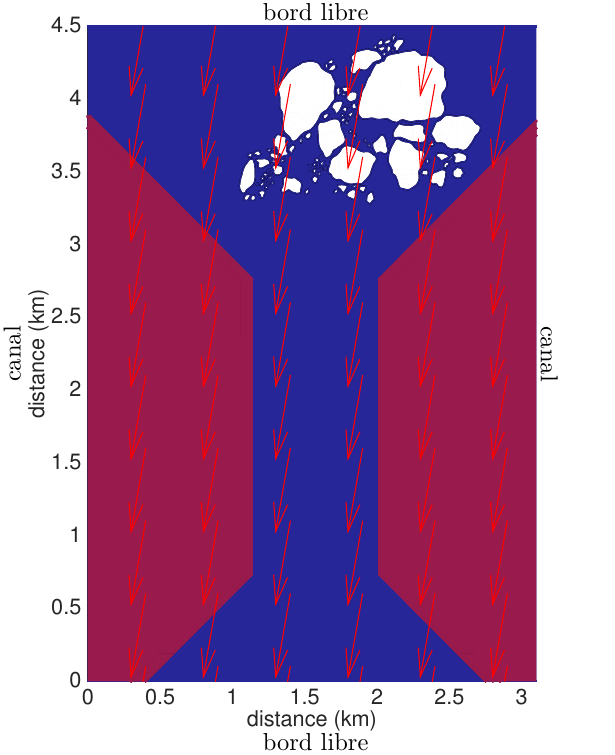
\includegraphics[width=.28\textwidth]{Derive.png}
    \caption{Configuration à l’instant initial pour le scénario de dérive dans un canal étroit \parencite[p.124]{rabatel2015thesis}.}
    \label{fig:Derive}
\end{figure}

\begin{figure}[!h]
    \centering
    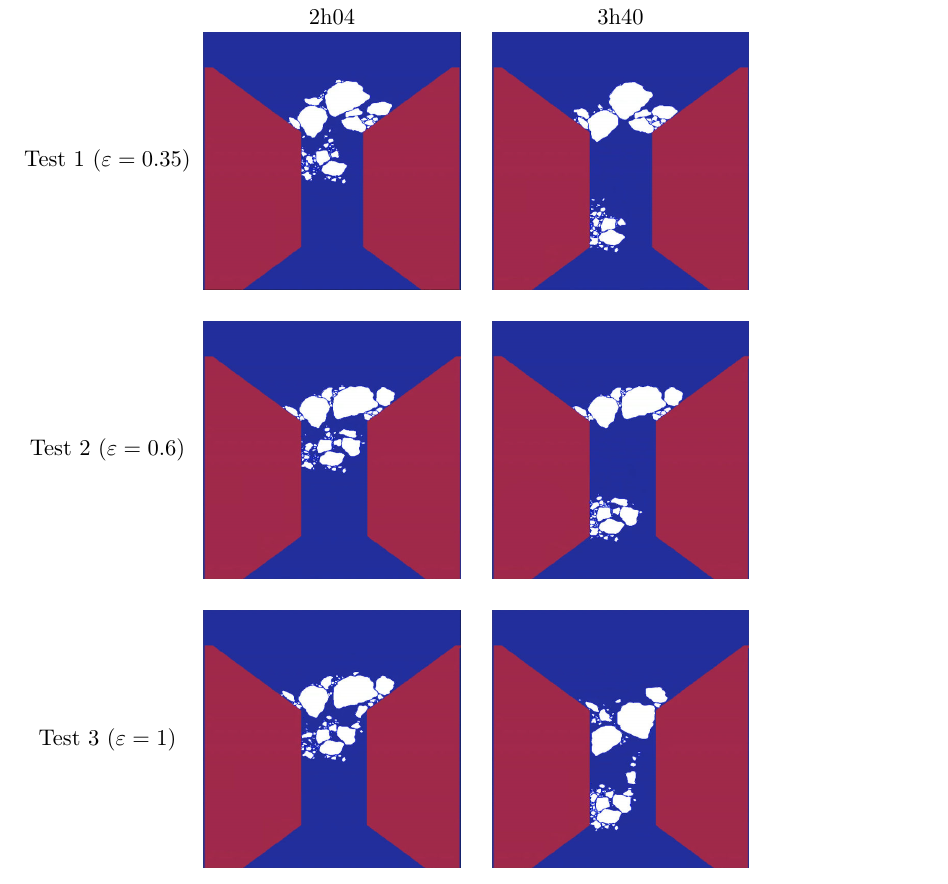
\includegraphics[width=.68\textwidth]{DeriveSol.png}
    \caption{Quelques résultats obtenus à deux heures différentes de la configuration des floes pour différentes valeurs du coefficient de restitution $\varepsilon$ \parencite[p.126]{rabatel2015thesis}.}
    \label{fig:DeriveSol}
\end{figure}

\subsection{Discussion}
Bien que les travaux de \citeauthor{rabatel2015thesis} ont été testés et validés sur plusieurs configurations différentes, il reste néanmoins des points qui ne sont pas traités, et qui ont très clairement été soulignés dans la thèse \parencite{rabatel2015thesis} :
\begin{enumerate}
    \item Le modèle ne gère pas la rhéologie\footnote{La rhéologie est l'étude de la déformation et de l'écoulement de la matière sous l'effet d'une contrainte appliquée.} de la glace : les floes sont des solides purement rigides (ils ne se déforment pas) et la dissipation d’énergie cinétique durant la collision est décrite en utilisant un coefficient purement empirique collision.  
    \item La loi de contact utilisée pour le glissement (voir \parencite{stewart1996implicit}), bien que très riche, ne prends pas en compte toutes les vitesses possibles de déplacement. La construction d’une loi qui donnerait accès à la région entière, demanderait de prendre en compte un grand nombre de phénomènes intrinsèques aux contacts. Leur compréhension et leur rôle à chacun est difficile à déterminer. 
    \item Les coefficients de friction et de restitution utilisées sont limitants. En réalité, il n’est pas possible de prendre en compte ou d'interpréter mathématiquement certains effets lors du contact ; par exemple, avec la dispersion de l'énergie (voir \parencite{nguyen2014multiple}). Cette dispersion est la conséquence de certains effets vibratoires à travers une chaîne de contact. Seuls les effets de dissipation dus aux phénomènes locaux comme l’endommagement, la viscosité ou la plasticité sont pris en compte à travers l’utilisation des coefficients de restitution et de friction.
    \item Les vitesses obtenues après la phase de décompression afin d'assurer la dissipation de l'énergie cinétique possèdent une faiblesse : elles ne sont solutions que sous certaines conditions, comme le fait que les chocs soient frontaux et qu’il n’y ait pas d’apport des forces extérieures autres que les forces de contact durant la collision \parencite[p.41]{rabatel2015thesis}.
\end{enumerate}

